\documentclass{beamer}
\usetheme{Madrid}
\usecolortheme{default}

\usepackage[utf8]{inputenc}
\usepackage{amsmath,amssymb}   % math symbols
% \usepackage{bm}                 % bold math vectors
\usepackage{xcolor}             % colors
\usepackage{graphicx}           % images
\usepackage{listings}           % code listing
\usepackage{courier}    % monospace font for code
\usepackage{gvv}

% Optional: customize Python highlighting in listings
\lstset{
    language=Python,
    basicstyle=\ttfamily\small,       % font and size
    keywordstyle=\color{blue},
    stringstyle=\color{orange},
    commentstyle=\color{green!60!black},
    showstringspaces=false,
    breaklines=true,
    numbers=left,
    numberstyle=\tiny\color{gray},
    frame=single,                     % frame around code
    tabsize=4
}

\lstset{
    language=C,
    basicstyle=\ttfamily\small,
    keywordstyle=\color{blue},
    stringstyle=\color{orange},
    commentstyle=\color{green!60!black},
    numbers=left,
    numberstyle=\tiny\color{gray},
    breaklines=true,
    showstringspaces=false,
}


\title{8.4.34}
\author{Sai Sreevallabh - EE25BTECH11031}


\begin{document}

\frame{\titlepage}

\begin{frame}{Question}
Let $\brak{x,y}$, be any point on the parabola $y^2 = 4x$. Let $\vec{P}$ be the point that divides the line segment from $\brak{0,0}$ to $\brak{x,y}$ in the ration 1:3. Then the locus of $\vec{P}$ is.
\begin{enumerate}
    \item $x^2 = y$
    \item $y^2 = 2x$
    \item $y^2 = x$
    \item $x^2 = 2y$
\end{enumerate}

\end{frame}

\begin{frame}{Theoretical Solution}

Given points can be taken to be
\begin{align}
    \vec{O} = \myvec{0\\0} \ \text{and} \ \vec{Q} = \myvec{x\\y}
\end{align}

Point $\vec{P} = \myvec{x_p\\y_p}$ divides the line segment $\vec{P-O}$ in the ratio 1:3. so
\begin{align}
    \vec{P} = \frac{3\vec{O}+\vec{Q}}{3+1}\\
    \implies \myvec{x_p\\y_p} = \frac{1}{4}\myvec{x\\y}
\end{align}

\end{frame}

\begin{frame}{Theoretical Solution}

So, 
\begin{align}
    x = 4x_p \ \ \text{and} \ \ y = 4y_p
\end{align}

Substituting the above in the equation in the parabola $y^2 = 4x$.
\begin{align}
    y_p^2 = x_p
\end{align}

Therefore, the locus of the point $\vec{P}$ is the parabola $y^2 = x$. 

\end{frame}

\begin{frame}[fragile]
    \frametitle{C Code}

    \begin{lstlisting}
#include <stdio.h>

void compute_parabola(double *y, double *x, int n) {
    for (int i = 0; i < n; i++) {
        x[i] = (y[i] * y[i]) / 4.0;
    }
}

    \end{lstlisting}

\end{frame}


\begin{frame}[fragile]
    \frametitle{Python Code - Using Shared Object}
    \begin{lstlisting}
import numpy as np
import matplotlib.pyplot as plt
import ctypes

c_lib=ctypes.CDLL("./code.so")

c_lib.compute_parabola.argtypes = [
    ctypes.POINTER(ctypes.c_double),
    ctypes.POINTER(ctypes.c_double),
    ctypes.c_int
]

y = np.linspace(-5,5,100)
x = np.zeros_like(y)


\end{lstlisting}
\end{frame}

\begin{frame}[fragile]
    \frametitle{Python Code - Using Shared Object}
    \begin{lstlisting}


c_lib.compute_parabola(
    y.ctypes.data_as(ctypes.POINTER(ctypes.c_double)),
    x.ctypes.data_as(ctypes.POINTER(ctypes.c_double)),
    y.size
)

plt.plot(x, y, color = 'red' ,label = "$y^2 = 4x$")

x_p = (3*0 + x)/(3+1)
y_p = (3*0 + y)/(3+1)

plt.plot([0,1], [0,2], color = 'black')
plt.scatter([0,1,0.25], [0,2,0.5])

plt.plot(x_p, y_p, color = 'green', label = "$y^2 = x$")

\end{lstlisting}
\end{frame}

\begin{frame}[fragile]
    \frametitle{Python Code - Using Shared Object}
    \begin{lstlisting}
    
ax = plt.gca()
ax.spines['top'].set_color('none')
ax.spines['bottom'].set_position('zero')
ax.spines['right'].set_color('none')
ax.spines['left'].set_position('zero')
plt.xlabel('x')
plt.ylabel('y')
plt.legend(loc='best')
plt.grid(False)
plt.axis('equal')
plt.xlim(-2, 2)
plt.ylim(-4, 4)

\end{lstlisting}
\end{frame}

\begin{frame}{Plot-Using Both C and Python}
    \centering
    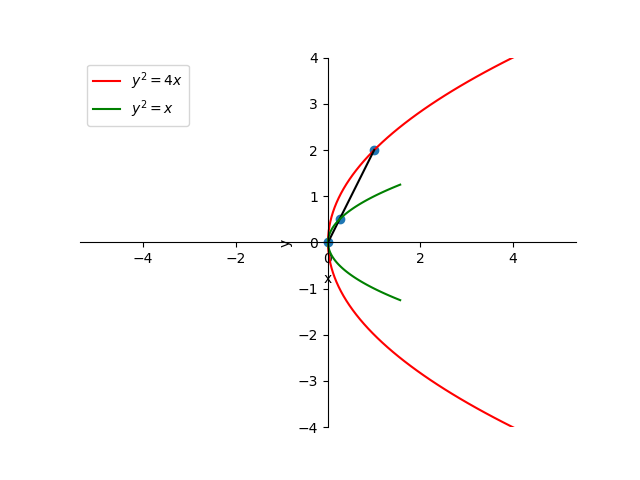
\includegraphics[width=\columnwidth, height=0.8\textheight, keepaspectratio]{Figs/plot(py+C).png}     
\end{frame}

%-------End of Python+C-------------


\begin{frame}[fragile]
    \frametitle{Python Code}
    \begin{lstlisting}
import numpy as np
import matplotlib.pyplot as plt
import math

y = np.linspace(-8, 8, 1000)

x = (y*y)/4

plt.plot(x, y, label = "$y^2 = 4x$")

x_p = (3*0 + x)/(3+1)
y_p = (3*0 + y)/(3+1)

plt.plot([0,1], [0,2])
plt.scatter([0,1,0.25], [0,2,0.5])

plt.plot(x_p, y_p, label = "$y^2 = x$")

\end{lstlisting}
\end{frame}

\begin{frame}[fragile]
    \frametitle{Python Code}
    \begin{lstlisting}
ax = plt.gca()
ax.spines['top'].set_color('none')
ax.spines['bottom'].set_position('zero')
ax.spines['right'].set_color('none')
ax.spines['left'].set_position('zero')
plt.xlabel('x')
plt.ylabel('y')
plt.legend(loc='best')
plt.grid(False)
plt.axis('equal')
plt.xlim(-2, 2)
plt.ylim(-4, 4)


plt.savefig("../Figs/plot(py).png")
plt.show()

\end{lstlisting}
\end{frame}


\begin{frame}{Plot-Using Python only}
    \centering
    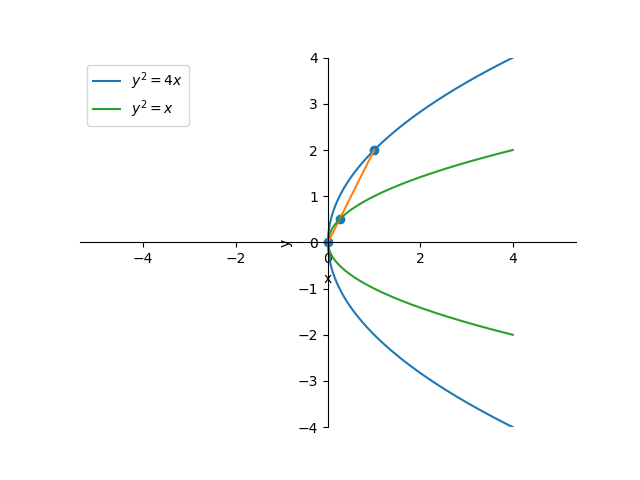
\includegraphics[width=\columnwidth, height=0.8\textheight, keepaspectratio]{Figs/plot(py).png}     
\end{frame}


\end{document}

